\newpage
\appendix
\section{Technical Reference: Algorithms, Diagrams, and Source Code}
\label{appendix:technical_reference}

The following sections contain the comprehensive technical blueprints for the primary spatial computing protocols discussed in the Methodology. This includes the formal algorithmic logic, high-level system orchestration diagrams, and the raw JavaScript client-side implementations that manage WebGL canvas isolation and asynchronous data transmission.

\subsection{A.1 Generative Extraction and Deep Splat Excavation (DBSE)}

The interactive selection protocol bypasses computationally expensive 3D raycasting by utilizing a 2D viewport slicing mechanism. The formal execution logic for this extraction is defined in Algorithm \ref{alg:dbse_interaction}.

\begin{algorithm}[H]
\caption{Client-Side Bounding Box Extraction and Mesh Injection Protocol}
\label{alg:dbse_interaction}
\begin{algorithmic}[1]
\Require User selection box $B_{2D} = (x, y, w, h)$, Camera Matrix $C$, 3D Scene $S$
\Ensure Transmitted viewport slice $I_{crop}$ and injected 3D mesh $M_{glb}$
\State \textbf{Initialize} interactive 2D canvas overlay linked to mouse coordinates
\If{Mouse drag event detected}
    \State Update $B_{2D} \leftarrow$ dynamic $(x, y, w, h)$ bounds
    \State Render selection rectangle on overlay
\EndIf
\If{Mouse release event detected}
    \State Disable $S$ environmental variables (fog, grid, ambient light)
    \State Render clean, unobstructed frame of $S$
    \State Map $B_{2D}$ bounds to absolute WebGL pixel coordinates $(p_x, p_y, p_w, p_h)$
    \State $I_{crop} \leftarrow$ Extract pixels from canvas buffer at mapped coordinates
    \State Restore $S$ environmental variables
    \State \textbf{Transmit} $I_{crop}$ payload to /api-fastapi/extract via POST
    \State \textbf{Await} HTTP Response $\rightarrow$ ArrayBuffer $A_{glb}$
    \State $M_{glb} \leftarrow$ Parse GLTF geometry from $A_{glb}$
    \State Calculate target centroid $C_{target}$ derived from $C$ forward vector
    \State Translate $M_{glb}$ to $C_{target}$ and apply maximum dimension normalization
    \State Inject $M_{glb}$ into $S$ and update rendering loop
\EndIf
\end{algorithmic}
\end{algorithm}

\vspace{0.5cm}
Figure \ref{fig:imgto3d} outlines the high-level semantic segmentation and extraction pipeline for this process, while Figure \ref{fig:dbselogo} visualizes the localized Z-buffer depth analysis utilized to execute the non-destructive spatial mask. 

% CHANGED TO [H] TO GLUE THE IMAGE EXACTLY HERE
\begin{figure}[H] 
    \centering
    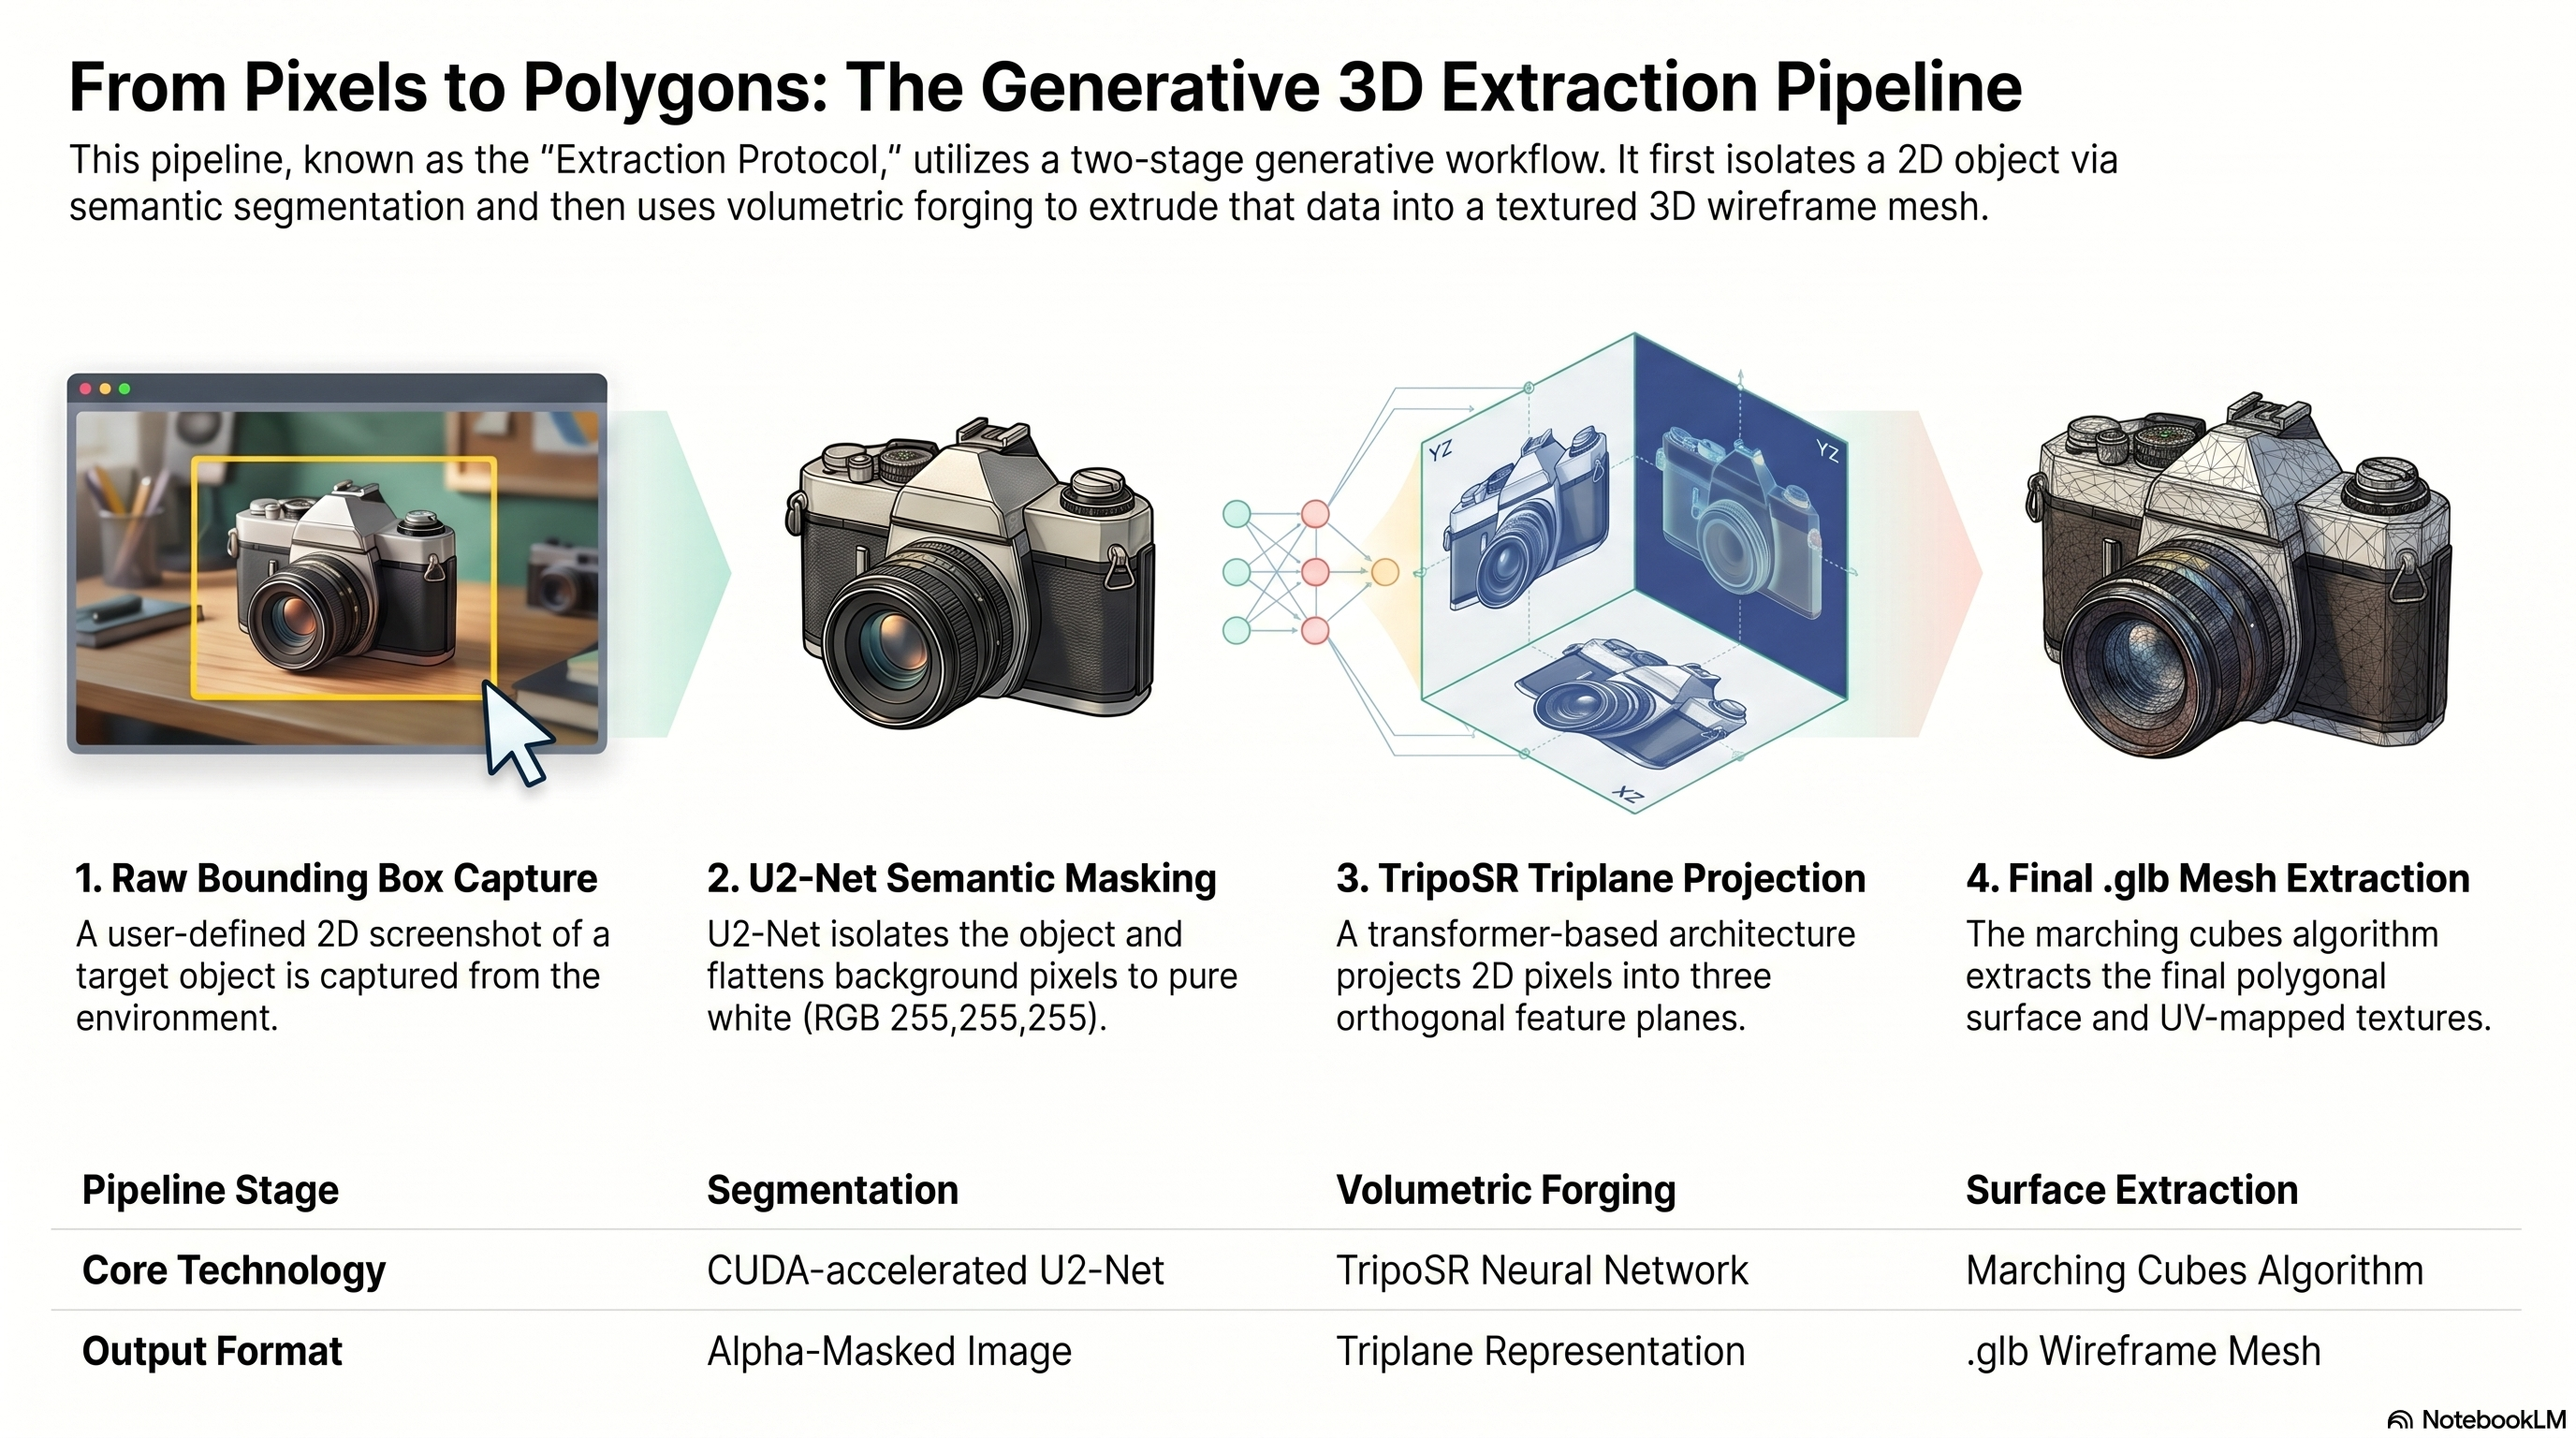
\includegraphics[width=\linewidth]{img/11.png}
    \caption{Created by NotebookLM - The Generative 3D Extraction Pipeline (Scenario 1). This sequential flowchart illustrates the transformation of a raw 2D viewport selection into a fully textured 3D model. The process details the initial semantic segmentation via U\textsuperscript{2}-Net (enforcing a pure white background), followed by volumetric forging and surface extraction utilizing the TripoSR neural network and the marching cubes algorithm.}
    \label{fig:imgto3d}
\end{figure}

% CHANGED TO [H] TO GLUE THE IMAGE EXACTLY HERE
\begin{figure}[H] 
    \centering
    \includegraphics[width=\linewidth]{img/12.png}
    \caption{Created by NotebookLM - The Deep Splat Excavation "hole-punch" process. This overlay demonstrates the mathematical translation of a 2D user selection into a 3D volumetric mask, allowing new assets to be spawned without visual clipping or Z-fighting with the original scanned environment.}
    \label{fig:dbselogo}
\end{figure}

\vspace{0.5cm}
The corresponding JavaScript implementation for this viewport capture protocol is provided in Listing \ref{lst:capture}.

\begin{lstlisting}[language=Java, caption={JavaScript Implementation of captureSelectionSnapshot()}, label={lst:capture}]
function captureSelectionSnapshot(bb) {
    try {
        const prevBg = scene.background ? scene.background.clone() : null;
        const prevFog = scene.fog;
        const prevGridVisible = gridHelper.visible;

        // Isolate canvas for clean extraction
        scene.background = new THREE.Color(0xffffff);
        scene.fog = null;
        gridHelper.visible = false;

        renderer.render(scene, camera);

        const srcCanvas = renderer.domElement;
        const rect = srcCanvas.getBoundingClientRect();
        
        // Map 2D bounds to WebGL coordinates
        const scaleX = srcCanvas.width / rect.width;
        const scaleY = srcCanvas.height / rect.height;
        const clampedW = Math.min(Math.round(bb.w * scaleX), srcCanvas.width);
        const clampedH = Math.min(Math.round(bb.h * scaleY), srcCanvas.height);

        const offCanvas = document.createElement('canvas');
        offCanvas.width = clampedW;
        offCanvas.height = clampedH;
        const offCtx = offCanvas.getContext('2d');
        
        // Extract pixels
        offCtx.drawImage(srcCanvas, Math.round((bb.x - rect.left) * scaleX), Math.round((bb.y - rect.top) * scaleY), clampedW, clampedH, 0, 0, clampedW, clampedH);
        const dataURL = offCanvas.toDataURL('image/png');

        // Restore environment variables
        scene.background = prevBg;
        scene.fog = prevFog;
        gridHelper.visible = prevGridVisible;
        renderer.render(scene, camera);

        // Transmit to FastAPI Backend
        fetch('/api-fastapi/extract', {
            method: 'POST',
            headers: { 'Content-Type': 'application/json' },
            body: JSON.stringify({ image: dataURL })
        }).then(response => response.arrayBuffer())
          .then(arrayBuffer => {
              // Parse and inject generated GLB mesh
              const loader = new GLTFLoader();
              loader.parse(arrayBuffer, '', (gltf) => {
                  scene.add(gltf.scene);
              });
          });
    } catch (err) {
        console.error('[SYSTEM_ERR] Snapshot failed:', err.message);
    }
}
\end{lstlisting}

\newpage
\subsection{A.2 The Summoning Engine: Text-to-3D Orchestration}

Operating heavy generative models strictly within an 8GB VRAM constraint requires the aggressive memory management strategy depicted in Figure \ref{fig:txt23d}. 

% CHANGED TO [H] TO GLUE THE IMAGE EXACTLY HERE
\begin{figure}[H] 
    \centering
    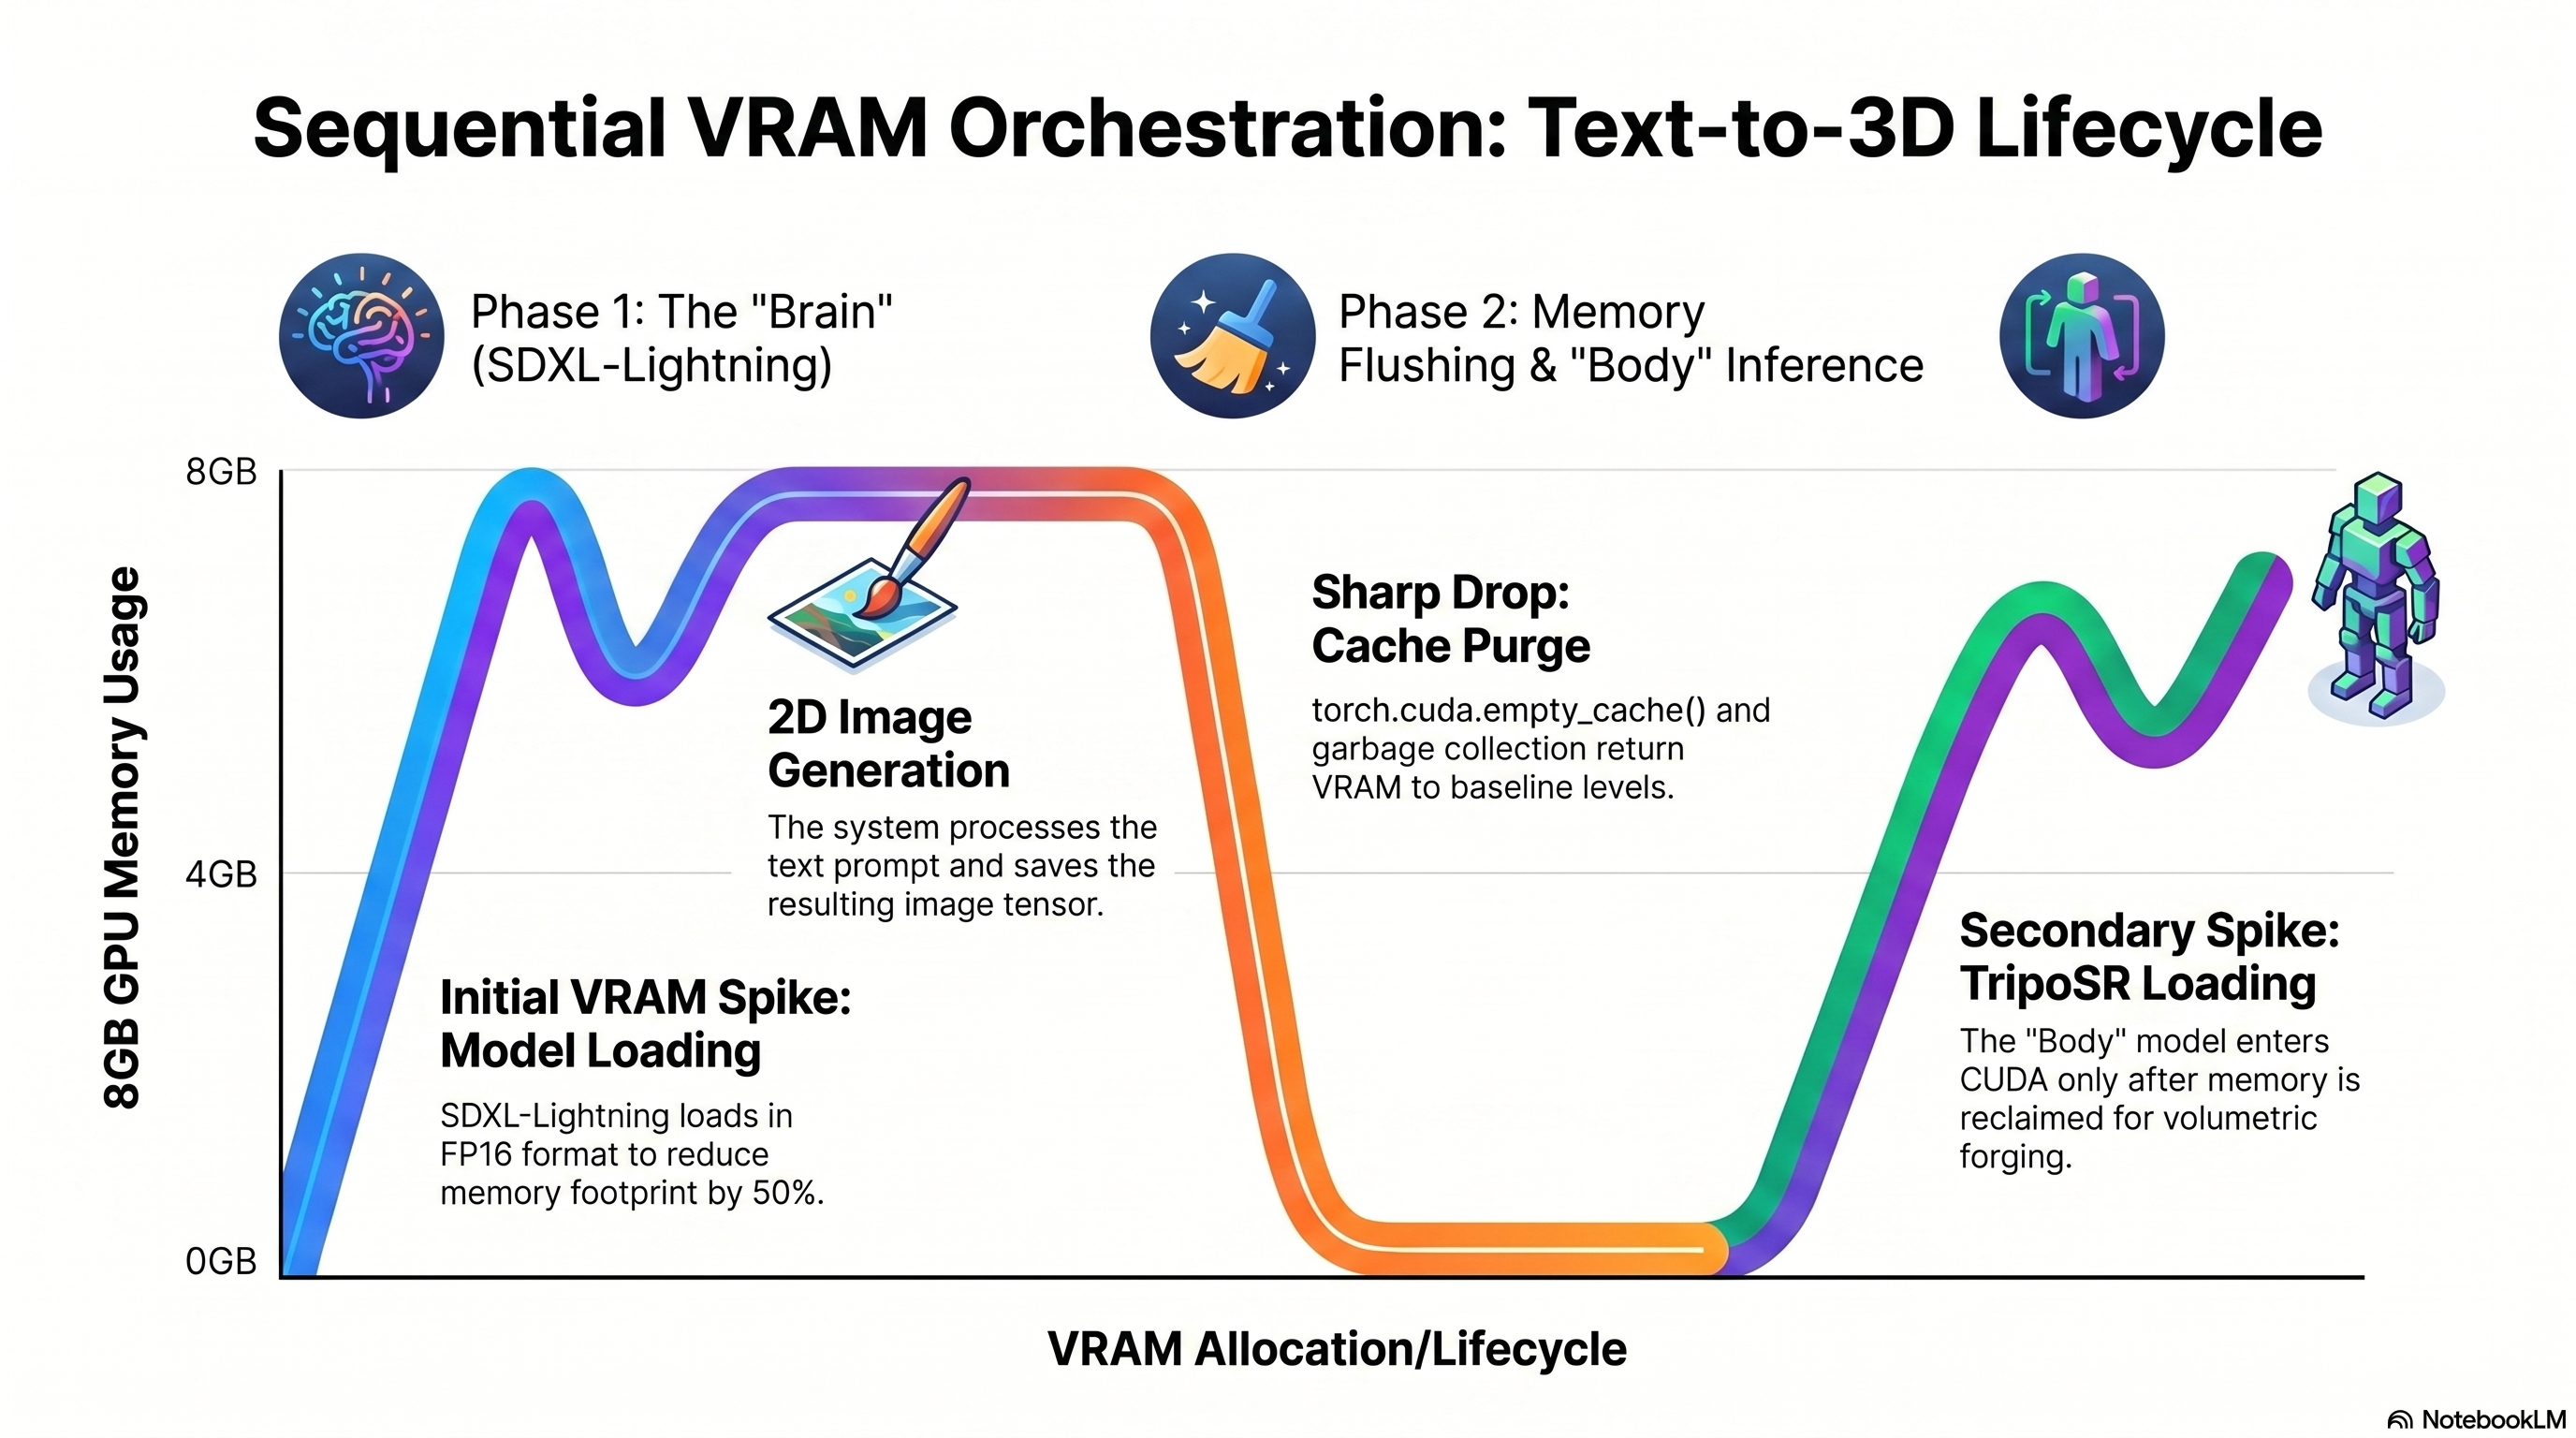
\includegraphics[width=\linewidth]{img/13.png}
    \caption{Created by NotebookLM - Sequential VRAM Orchestration during the Text-to-3D Lifecycle. The graph demonstrates the aggressive memory management strategy required to operate within an 8GB GPU threshold. It highlights the initial VRAM spike during SDXL-Lightning inference, the critical cache purge (\texttt{torch.cuda.empty\_cache()}), and the subsequent memory reallocation for TripoSR volumetric forging.}
    \label{fig:txt23d}
\end{figure}

\vspace{0.5cm}
The asynchronous client-side fetch requests and geometry parsing functions handling this orchestration are detailed in Listing \ref{lst:summon}.

\begin{lstlisting}[language=Java, caption={JavaScript Implementation of executePromptSummon()}, label={lst:summon}]
function executePromptSummon() {
    const prompt = creatorPromptInput.value.trim();
    if (!prompt) return;
    
    showCreatorLoader('Connecting to Stable Diffusion SD3 generator...', 15);
    
    fetch('/api-proxy/summon', {
        method: 'POST',
        headers: { 'Content-Type': 'application/json' },
        body: JSON.stringify({ prompt: prompt })
    })
    .then(response => {
        if (!response.ok) throw new Error(`HTTP ${response.status}`);
        showCreatorLoader('Image generated. Forging 3D geometry locally via TripoSR...', 55);
        return response.arrayBuffer();
    })
    .then(arrayBuffer => {
        showCreatorLoader('Reconstruction complete. Loading 3D spatial mesh...', 85);
        
        const loader = new GLTFLoader();
        loader.parse(arrayBuffer, '', (gltf) => {
            const model = gltf.scene;
            
            // Calculate target spawn point derived from camera forward vector
            const forward = new THREE.Vector3();
            camera.getWorldDirection(forward);
            const targetPos = new THREE.Vector3().copy(camera.position).addScaledVector(forward, 5);
            model.position.copy(targetPos);
            
            // Hide Gaussian Splat environment to reveal standalone mesh
            if (viewer && viewer.splatMesh) viewer.splatMesh.visible = false;
            
            scene.add(model);
            hideCreatorLoader();
        });
    })
    .catch(err => {
        console.error('SYS_ERR: Summon failed:', err.message);
        hideCreatorLoader();
    });
}
\end{lstlisting}